% Left: a colouring of K5 with no monochromatic triangle. Right: a random colouring of K6 with a monochromatic triangle. Generated by a short script.
% Pale inks are 55 percent of the series colours mixed with white, as opaque
% RGB, so this plate does not put a transparency group on the text page.
\definecolor{ocRustPale}{HTML}{CC978E}
\definecolor{ocCharPale}{HTML}{7E7E7F}
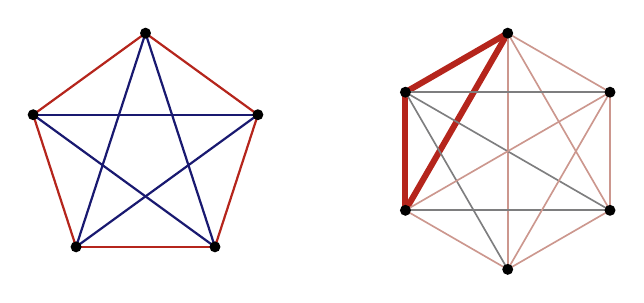
\begin{tikzpicture}[v/.style={circle,fill=black,inner sep=1.4pt}]
\draw[BrickRed,thick] (0.000,1.500)--(-1.427,0.464);
\draw[MidnightBlue,thick] (0.000,1.500)--(-0.882,-1.214);
\draw[MidnightBlue,thick] (0.000,1.500)--(0.882,-1.214);
\draw[BrickRed,thick] (0.000,1.500)--(1.427,0.464);
\draw[BrickRed,thick] (-1.427,0.464)--(-0.882,-1.214);
\draw[MidnightBlue,thick] (-1.427,0.464)--(0.882,-1.214);
\draw[MidnightBlue,thick] (-1.427,0.464)--(1.427,0.464);
\draw[BrickRed,thick] (-0.882,-1.214)--(0.882,-1.214);
\draw[MidnightBlue,thick] (-0.882,-1.214)--(1.427,0.464);
\draw[BrickRed,thick] (0.882,-1.214)--(1.427,0.464);
\node[v] at (0.000,1.500) {};
\node[v] at (-1.427,0.464) {};
\node[v] at (-0.882,-1.214) {};
\node[v] at (0.882,-1.214) {};
\node[v] at (1.427,0.464) {};
\draw[BrickRed,line width=2.2pt] (4.600,1.500)--(3.301,0.750);
\draw[BrickRed,line width=2.2pt] (4.600,1.500)--(3.301,-0.750);
\draw[ocRustPale,semithick] (4.600,1.500)--(4.600,-1.500);
\draw[ocRustPale,semithick] (4.600,1.500)--(5.899,-0.750);
\draw[ocRustPale,semithick] (4.600,1.500)--(5.899,0.750);
\draw[BrickRed,line width=2.2pt] (3.301,0.750)--(3.301,-0.750);
\draw[ocCharPale,semithick] (3.301,0.750)--(4.600,-1.500);
\draw[ocCharPale,semithick] (3.301,0.750)--(5.899,-0.750);
\draw[ocCharPale,semithick] (3.301,0.750)--(5.899,0.750);
\draw[ocRustPale,semithick] (3.301,-0.750)--(4.600,-1.500);
\draw[ocCharPale,semithick] (3.301,-0.750)--(5.899,-0.750);
\draw[ocRustPale,semithick] (3.301,-0.750)--(5.899,0.750);
\draw[ocRustPale,semithick] (4.600,-1.500)--(5.899,-0.750);
\draw[ocRustPale,semithick] (4.600,-1.500)--(5.899,0.750);
\draw[ocRustPale,semithick] (5.899,-0.750)--(5.899,0.750);
\node[v] at (4.600,1.500) {};
\node[v] at (3.301,0.750) {};
\node[v] at (3.301,-0.750) {};
\node[v] at (4.600,-1.500) {};
\node[v] at (5.899,-0.750) {};
\node[v] at (5.899,0.750) {};
\end{tikzpicture}
